\section{Boolean Operations on Sets}

\subsubsection{Unions: $A\cup B$}
The union of two sets results in a set that contains all things belonging to either set.

\begin{example}The set of all negative integers unioned with the set of all positive integers and zero is the set of all integers.
\end{example}

\begin{example}
$A = \{1, 3, 5  \}$ and $B = \{ 10, 4\}$.  Then $A\cup B = \{1, 3, 4, 5, 10 \}$.\end{example}


\subsubsection{Intersections: $A\cap B$}
The intersection of two sets is the set of elements that are contained in both sets (or \emph{common} to both sets).


\begin{example}The intersection of the set of all negative integers unioned with the set of all positive integers and zero is the set of all integers is $\emptyset$.
\end{example}

\begin{example}
$A = \{1, 3, 5  \}$ and $B = \{ 1, 4, 6\}$.  Then $A\cap B = \{1\}$.\end{example}

\subsection*{Complementation}
Some people may refer to this as \emph{the inverse of discourse}.  This sort of means that there is some ``discourse'' going on.  I know that sounds vague, but really it will make sense.  If we are talking about planer geometry, then the set of intererest could be the points on the plane.  If we are talking about sociology, then the set could be all people.  For number theory, the set could be all natural numbers. In any case, the context will be made clear to you from the problem you are working on.  

Let us refer to the set, $I$  (i.e the set of all people might be $I$). 
\begin{definition}[Complement: $\overline A$]
For a set, $A\subset I$, the complement of $A$ is the set of all elements of $I$ that are not in $A$.  
\end{definition}
\begin{example}
Let $I$ be the set of all natural numbers and $A\subset I$ is the set of all even natural numbers.  Then $\overline A$ is the set of all odd natural numbers.
\end{example}
\begin{remark} [$\overline{\overline{A}} = A$]
\end{remark}

Final comment:  These operations, union, intersection and complementation, are the fundamental operations on sets (Boolean operations).  We can define other operations in terms of these. 
\begin{example}[$A-B$]
The difference of two sets, $A-B$, can be expressed as $A\cap \overline B$.
\end{example}

\newpage
\subsection*{Venn Diagrams}
A great way to visualize the Boolean operations on a set is by using Venn Diagrams.   Below are some illustrations of how the operations can be represented.
%\begin{tikzpicture}
%% left hand
%\scope [fill=gray, opacity=0.5]
%\clip (-2,-2) rectangle (2,2)
%      (1,0) circle (1);
%\fill (0,0) circle (1);
%\endscope
%% right hand
%\scope[fill=gray, opacity=0.5]
%\clip (-2,-2) rectangle (2,2)
%      (0,0) circle (1);
%\fill (1,0) circle (1);
%\endscope
%% outline
%\draw (0,0) circle (1) (0,1)  node [text=black,above] {$A$}
%      (1,0) circle (1) (1,1)  node [text=black,above] {$B$}
%      (-2,-2) rectangle (3,2) node [text=black,above] {$H$};
%\end{tikzpicture}

%
%
%\def\firstcircle{(0,0) circle (1.5cm)}
%\def\secondcircle{(60:2cm) circle (1.5cm)}
%\def\thirdcircle{(0:2cm) circle (1.5cm)}
%\begin{tikzpicture}
%    \begin{scope}[shift={(3cm,-5cm)}, fill opacity=0.05]
%        \fill[red, opacity=0.05] \firstcircle;
%        \fill[green] \secondcircle;
%        \fill[blue] \thirdcircle;
%        \draw \firstcircle node[below] {$A$};
%        \draw \secondcircle node [above] {$B$};
%        \draw \thirdcircle node [below] {$C$};
%    \end{scope}
%\end{tikzpicture}
%
%
%\begin{tikzpicture}
% \begin{scope}[blend group=soft light] 
%%\begin{scope} [opacity=0.5]
%     \fill[red!30!white, fill opacity=0.5]   ( 90:1.2) circle (2);
%    \fill[green!30!white, fill opacity=0.5] (210:1.2) circle (2);
%    \fill[blue!30!white, fill opacity=0.5]  (330:1.2) circle (2);
% \end{scope}
%%  \node at ( 90:2)    {Typography};
%%  \node at (210:2)    {Design};
%%  \node at (330:2)    {Coding};
%%  \node [font=\Large] {\LaTeX};
%\end{tikzpicture}
%



% Definition of circles
\def\firstcircle{(0,0) circle (1.5cm)}
\def\secondcircle{(0:2cm) circle (1.5cm)}

\colorlet{circle edge}{black}
\colorlet{circle area}{blue!20}

\tikzset{filled/.style={fill=circle area, draw=circle edge, thick},
    outline/.style={draw=circle edge, thick}}

\setlength{\parskip}{5mm}
% Set A and B
\begin{tikzpicture}[scale=0.75]
    \begin{scope}
        \clip \firstcircle;
        \fill[filled] \secondcircle;
    \end{scope}
    \draw[outline] \firstcircle node {$A$};
    \draw[outline] \secondcircle node {$B$};
    \node[anchor=south] at (current bounding box.north) {$A \cap B$};
\end{tikzpicture}
%Set A or B but not (A and B) also known a A xor B
\begin{tikzpicture}[scale=0.75]
    \draw[filled, even odd rule] \firstcircle node {$A$}
                                 \secondcircle node{$B$};
    \node[anchor=south] at (current bounding box.north) {$\overline{A \cap B}$};
\end{tikzpicture}
% Set A or B
\begin{tikzpicture}[scale=0.75]
    \draw[filled] \firstcircle node {$A$}
                  \secondcircle node {$B$};
    \node[anchor=south] at (current bounding box.north) {$A \cup B$};
\end{tikzpicture}
% Set A but not B
\begin{tikzpicture}[scale=0.75]
    \begin{scope}
        \clip \firstcircle;
        \draw[filled, even odd rule] \firstcircle node {$A$}
                                     \secondcircle;
    \end{scope}
    \draw[outline] \firstcircle
                   \secondcircle node {$B$};
    \node[anchor=south] at (current bounding box.north) {$A - B$};
\end{tikzpicture}
% Set B but not A
\begin{tikzpicture}[scale=0.75]
    \begin{scope}
        \clip \secondcircle;
        \draw[filled, even odd rule] \firstcircle
                                     \secondcircle node {$B$};
    \end{scope}
    \draw[outline] \firstcircle node {$A$}
                   \secondcircle;
    \node[anchor=south] at (current bounding box.north) {$B - A$};
\end{tikzpicture}

\subsection*{Venn Diagrams for Three Sets}
This tool can be extended to include three sets in the following manner.

\begin{center}
\def\firstcircle{ (0.0, 0.0) circle (1.5)}
\def\secondcircle{(2.0, 0.0) circle (1.5)}
\def\thirdcircle{ (1.0,-1.5) circle (1.5)}
\def\rectangle{ (-1.5,-3.0) rectangle (3.5,1.0) }
\colorlet{circle edge}{black}
\colorlet{circle area}{blue!20}

\tikzset{filled/.style={fill=circle area, draw=circle edge, thick},
    outline/.style={draw=circle edge, thick}}

%\setlength{\parskip}{5mm}
%############################################################################
%############################################################################
%############################################################################
%\noindent
\begin{tikzpicture}[scale=0.75]
    \begin{scope}
        \clip  \firstcircle;
        \clip  \secondcircle;
        \fill[filled]   \thirdcircle ;
    \end{scope}
    \draw[outline] \firstcircle  node[left]  {$A$};
    \draw[outline] \secondcircle node[right] {$B$};
    \draw[outline] \thirdcircle  node[below] {$C$};
    \node[anchor=south] at (current bounding box.north) {$A \cap B \cap C$};
\end{tikzpicture} \qquad
%############################################################################
%############################################################################
%############################################################################
\begin{tikzpicture}[scale=0.75]
    \begin{scope}
        \clip \firstcircle \secondcircle \thirdcircle;
        \fill[filled]  \firstcircle \secondcircle \thirdcircle;
    \end{scope}
    \draw[outline] \firstcircle  node[left]  {$A$};
    \draw[outline] \secondcircle node[right] {$B$};
    \draw[outline] \thirdcircle  node[below] {$C$};
    \node[anchor=south] at (current bounding box.north) {$A \cup B \cup C$};
\end{tikzpicture} \qquad
%############################################################################
%############################################################################
%############################################################################
\begin{tikzpicture}[scale=0.75]
    \begin{scope}
        \clip \firstcircle;
        \fill[filled] \secondcircle;
    \end{scope}
    \draw[outline] \firstcircle  node[left]  {$A$};
    \draw[outline] \secondcircle node[right] {$B$};
    \draw[outline] \thirdcircle  node[below] {$C$};
    \node[anchor=south,align=center] at (current bounding box.north) 
      {$(A\cap B)=$\\$(A \cap B \cap C) + (A \cap B \cap C')$};
\end{tikzpicture} 
%############################################################################
%############################################################################
%############################################################################
\begin{tikzpicture}[scale=0.75]
    \begin{scope}
        \clip \firstcircle;
        \fill[filled] \thirdcircle;
    \end{scope}
    \begin{scope}
        \clip \firstcircle;
        \clip \secondcircle;
        \fill[white] \thirdcircle;
    \end{scope}
    \draw[outline] \firstcircle  node[left]  {$A$};
    \draw[outline] \secondcircle node[right] {$B$};
    \draw[outline] \thirdcircle  node[below] {$C$};
    \node[anchor=south] at (current bounding box.north) 
      {$(A\cap B' \cap C)$};
\end{tikzpicture} \qquad \\%[1.5cm]
%############################################################################
%############################################################################
%############################################################################
\begin{tikzpicture}[scale=0.75]
    \begin{scope}
        \fill[filled] \thirdcircle;
        \fill[white]  \firstcircle;
        \fill[white]  \secondcircle;
    \end{scope}
    \draw[outline] \firstcircle  node[left]  {$A$};
    \draw[outline] \secondcircle node[right] {$B$};
    \draw[outline] \thirdcircle  node[below] {$C$};
    \node[anchor=south] at (current bounding box.north) 
      {$(A' \cap B' \cap C)$};
\end{tikzpicture} \qquad
%############################################################################
%############################################################################
%############################################################################
\begin{tikzpicture}[scale=0.75]
     \begin{scope}
        \clip \secondcircle;
        \fill[filled] \thirdcircle;
    \end{scope}
    \fill[filled]  \firstcircle;
    \draw[outline] \firstcircle  node[left]  {$A$};
    \draw[outline] \secondcircle node[right] {$B$};
    \draw[outline] \thirdcircle  node[below] {$C$};
    \node[anchor=south] at (current bounding box.north) 
      {$A \cup (B \cap C)$};
\end{tikzpicture} %\\[1.5cm]
%############################################################################
%############################################################################
%############################################################################
\begin{tikzpicture}[scale=0.75]
     \begin{scope}
        \clip \firstcircle \secondcircle;
        \fill[filled] \thirdcircle;
    \end{scope}
    \draw[outline] \firstcircle  node[left]  {$A$};
    \draw[outline] \secondcircle node[right] {$B$};
    \draw[outline] \thirdcircle  node[below] {$C$};
    \node[anchor=south] at (current bounding box.north) 
      {$(A \cup B) \cap C$};
\end{tikzpicture} \qquad
\end{center}
For fun, we can see what the figure in the syllabus was implying,
\begin{center}
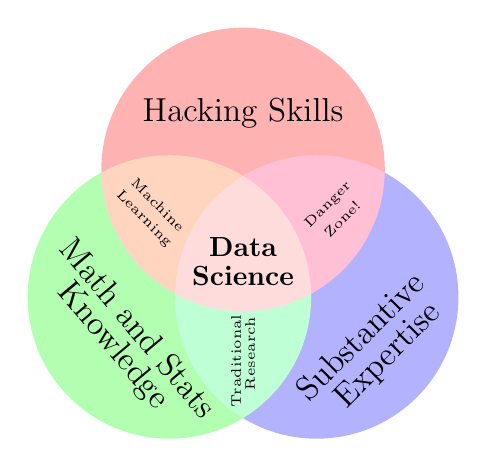
\begin{tikzpicture}[scale=0.9]
\begin{scope}[blend group=soft light]
  \fill[red!30!white]   ( 90:1.2) circle (2);
    \fill[green!30!white] (210:1.2) circle (2);
    \fill[blue!30!white]  (330:1.2) circle (2);
     \end{scope}
     
       \node at ( 90:2)    {\large Hacking Skills};
  \node[rotate=310] at (215:1.8)    {\large  Math and Stats};
  \node[rotate=310] at (215:2.25)    {\large Knowledge};
  \node[rotate=45]  at (325:2)    {\large Substantive};
  \node[rotate=45]  at (325:2.5)    {\large Expertise};
  \node at (90:0.1) {\bf Data};
  \node at (90:-0.3) {\bf Science};

  \node[rotate=45]  at (1.2,.7)    {\tiny Danger};
  \node[rotate=45]  at (1.4,0.5)    {\tiny Zone!};

  \node [rotate=90] at (-0.1,-1.5)    {\tiny Traditional};
  \node[rotate=90]  at (0.1,-1.4)    {\tiny Research};

  \node [rotate=-45] at (-1.2,0.7)    {\tiny Machine};
  \node[rotate=-45]  at (-1.4,0.5)    {\tiny Learning};
\end{tikzpicture}
\end{center}
